%----------------------------------------------------------------------------
\label{DC test section}
%----------------------------------------------------------------------------
%----------------------------------------------------------------------------
%----------------------------------------------------------------------------
%bb defines the bounding box for the pdf
%viewport defines the area of the pdf used
%in sidewaysfigure the last entry in bb moves the caption toward/away the pic
%in sidewaysfigure the second entry in bb moves the pic toward/away the caption
%----------------------------------------------------------------------------
\begin{figure}
\scalebox{0.8}[0.8]{
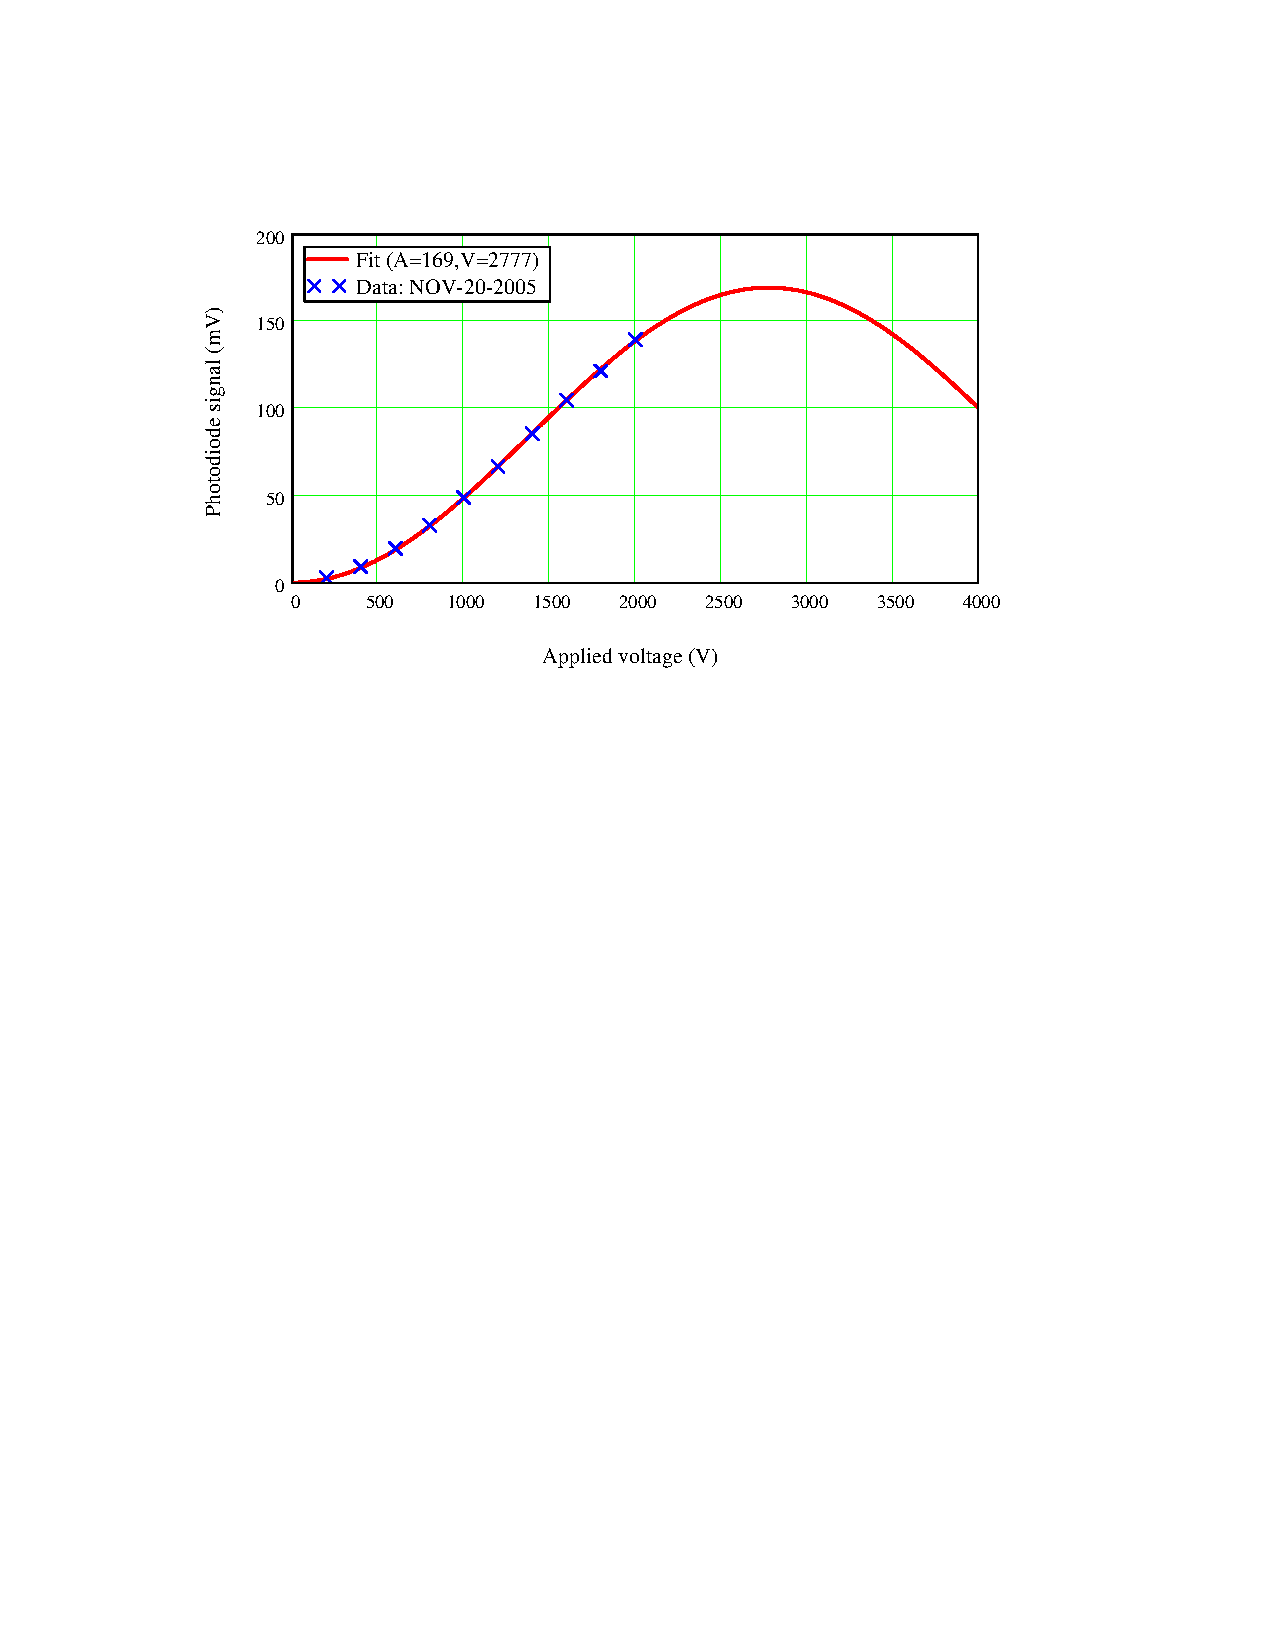
\includegraphics[bb=30 467 481 706]
{fit_628/fit_628.pdf}
}
\caption[DC test of 628nm coated Pockels cell]{DC test of 628nm coated Pockels cell. A base line photodiode reading (with the crossed polarizers and Pockels cell removed) was not recorded for these data; however, we expect the efficiency to be better than the green case in Figure \ref{fit_532} since the laser wavelength of 633nm is closer to AR coating wavelength.}
\label{fit_628}
\end{figure}
%----------------------------------------------------------------------------

%----------------------------------------------------------------------------
%bb defines the bounding box for the pdf
%viewport defines the area of the pdf used
%in sidewaysfigure the last entry in bb moves the caption toward/away the pic
%in sidewaysfigure the second entry in bb moves the pic toward/away the caption
%----------------------------------------------------------------------------
\begin{figure}
\scalebox{0.8}[0.8]{
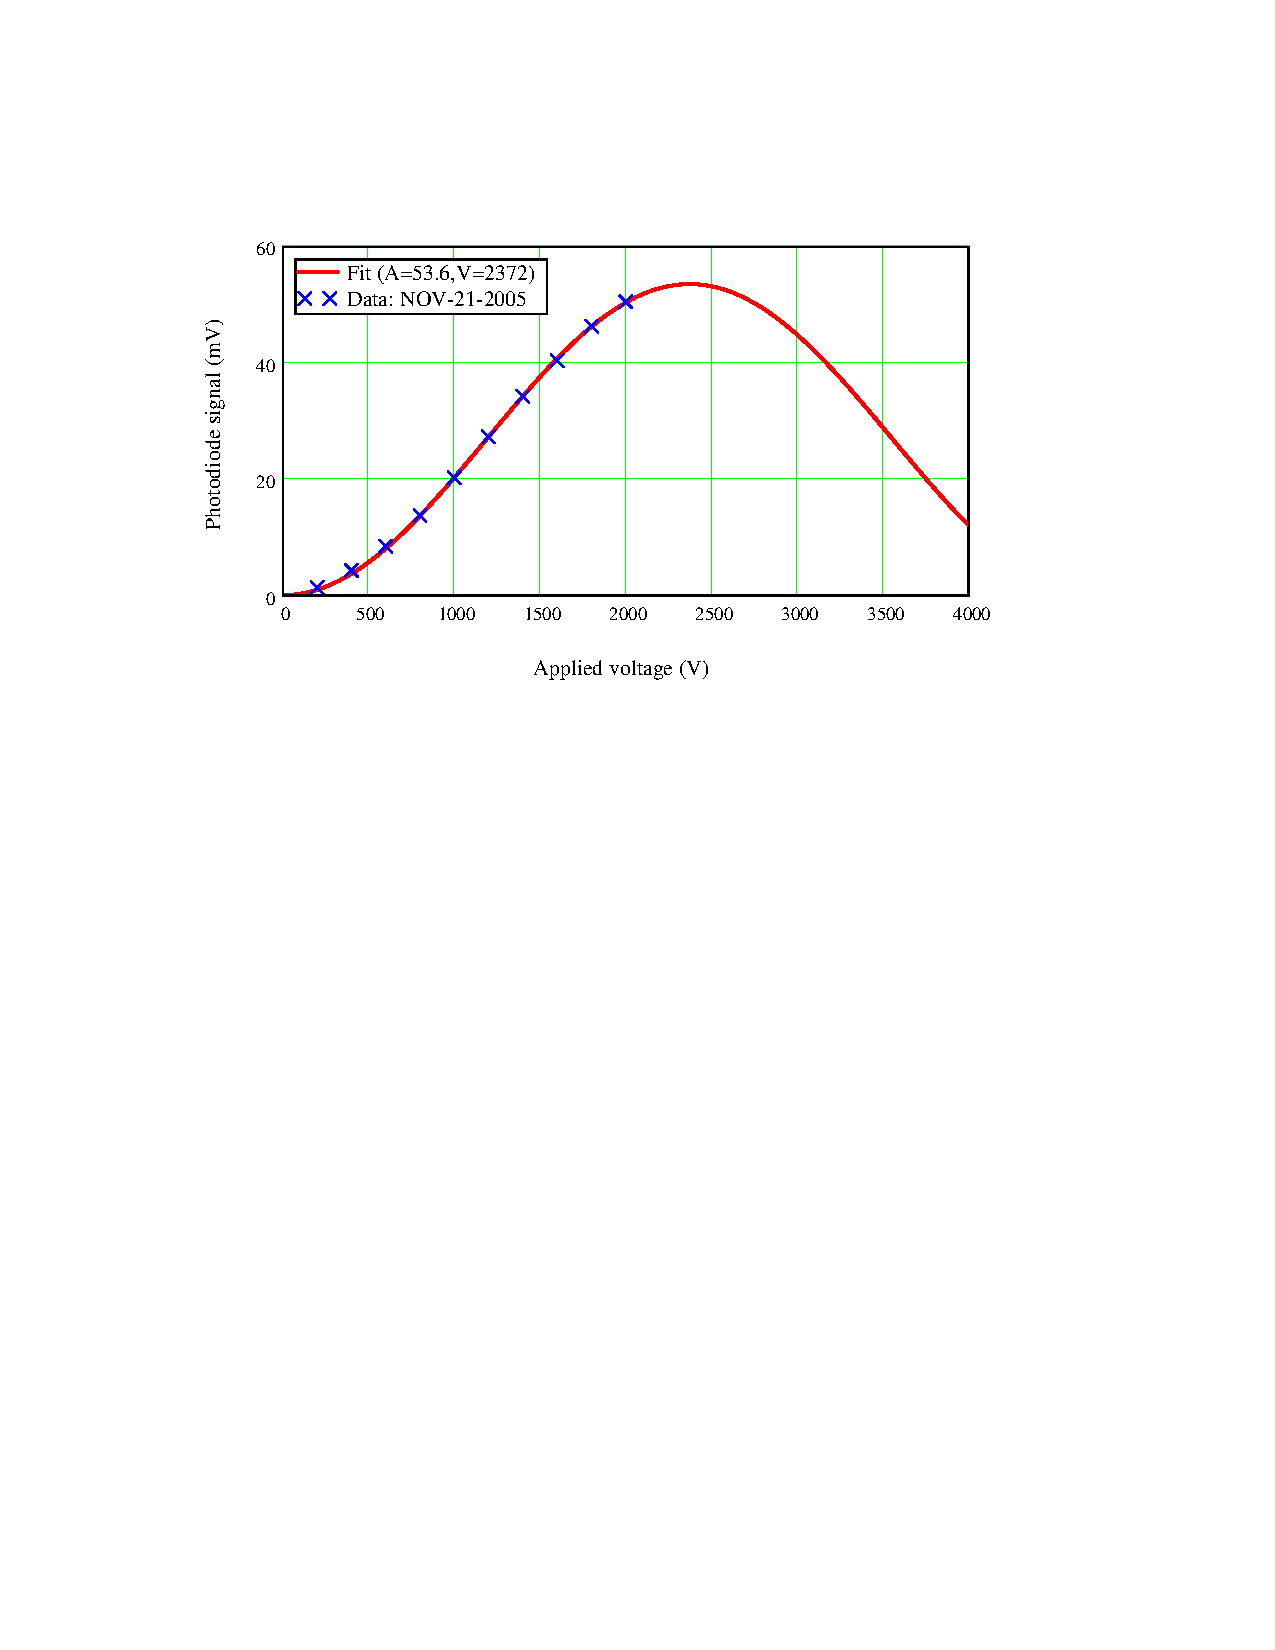
\includegraphics[bb=30 460 481 706]
{fit_532/fit_532.pdf}
}
\caption[DC test of 532nm coated Pockels cell]{DC test of 532nm coated Pockels cell. Since the photodiode signal is 76 mV with the crossed polarizers and Pockels cell removed, the fit value for A (53.6 mV) implies an efficiency of $e \sim 70\%$. Some of the attenuation may be due to the fact the laser wavelength of 543nm is different than the AR coating wavelength. The polarizers will also contribute to the attenuation factor for the system.}
\label{fit_532}
\end{figure}
%----------------------------------------------------------------------------

%----------------------------------------------------------------------------
Here we describe a test to determine a basic performance parameter of the Pockels cell: the applied voltage at which a beam passing through the cell will experience a 90 degree polarization rotation. By placing the Pockels cell between two crossed polarizers (10LP-VIS, Newport), the complete system (crossed polarizers and Pockels cell) becomes a light gate with respect to the applied voltage. If the cell is in a state where the polarization is not rotated, then light cannot pass through the system. However, if the Pockels cell rotates the beam polarization, significant power can begin to pass through the system. Maximum transmission occurs when the beam polarization is rotated 90$^\circ$. Specifically \cite{Saleh:1991a},
\begin{equation}
P_{out}
(V_a)
=
P_{in} e
\sin^2
\left(
\frac{\pi V_a}{2 V}
\right)
\label{power transmitted}
\end{equation}
where ${P_{out}}$ is the power downstream the system, $P_{in}$ is the power incident the system, $e$ is the efficiency of the system, $V_a$ is the applied voltage, and $V$ is the voltage at which maximum transmission occurs.

The mount for the Pockels cell provides delicate adjustment of the cell's orientation and clearance for the high voltage connectors. The Pockels cell is sensitive to yaw and pitch, requiring fine adjustment, while coarse adjustment of the roll angle and translation was sufficient. A transformer which increases the pulse height by a factor of two is placed close to the Pockels cell. The connection between the Pockels cell and the transformer is made using short wires about 2'' in length. This connection produces a lot of RF noise when the cell is run at high voltages and needs to be shielded to prevent interference with sensitive instruments. A simple tin foil shell was sufficient.

To determine the voltage at which the plane of polarization of a linearly polarized beam is rotated by 90$^\circ$ when run through the Pockels cell, a Hammarlung DC test power supply was used. A collimated CW green HeNe beam was chopped (50\% duty cycle at 200Hz) and sent through the crossed polarizer/Pockels cell system. A large area photodiode (Thorlabs PDA55) was used to detect the power transmitted through the system. A few ND filters were placed upstream the photodiode to select appropriate power levels for the diode. The output of the DC power supply was directly connected to the input terminals of the Pockels cell; thus, when the power supply's foot switch was depressed, the voltage applied to the Pockels cell could be read directly from the meter on the supply. Once the Pockels cell was activated in this manner, the corresponding voltage (representing the power transmitted through the system) from the photodiode could be observed using an oscilloscope.

The input beam to the Pockels cell was vertically polarized, while the Pockels cell was oriented so that the high voltage input terminals were horizontal (the terminals were at the ``9 o'clock'' position when facing downstream toward the cell). DC power supply voltages between 200V and 2000V were used in 200V steps. For each DC voltage applied to the Pockels cell, the corresponding voltage from the photodiode was recorded. A red HeNe was used for the Pockels cell coated for 628nm and a green HeNe was used for the 532nm coating. The data for each cell was fit to Equation \ref{power transmitted}. The coefficient $P_{in} e$ was fit as a single parameter $A$, so the efficiency of the system could be obtained indirectly by measuring the power incident the system and comparing it to the fit parameter $A$. See Figure \ref{fit_628} for the 628nm cell results, and Figure \ref{fit_532} for the 532nm results.

%----------------------------------------------------------------------------
%----------------------------------------------------------------------------
